
\chapter{Zrzuty ekranu interfejsu użytkownika}
\label{appendix:appScreenShots}

\begin{figure}[ht]
  \centering
  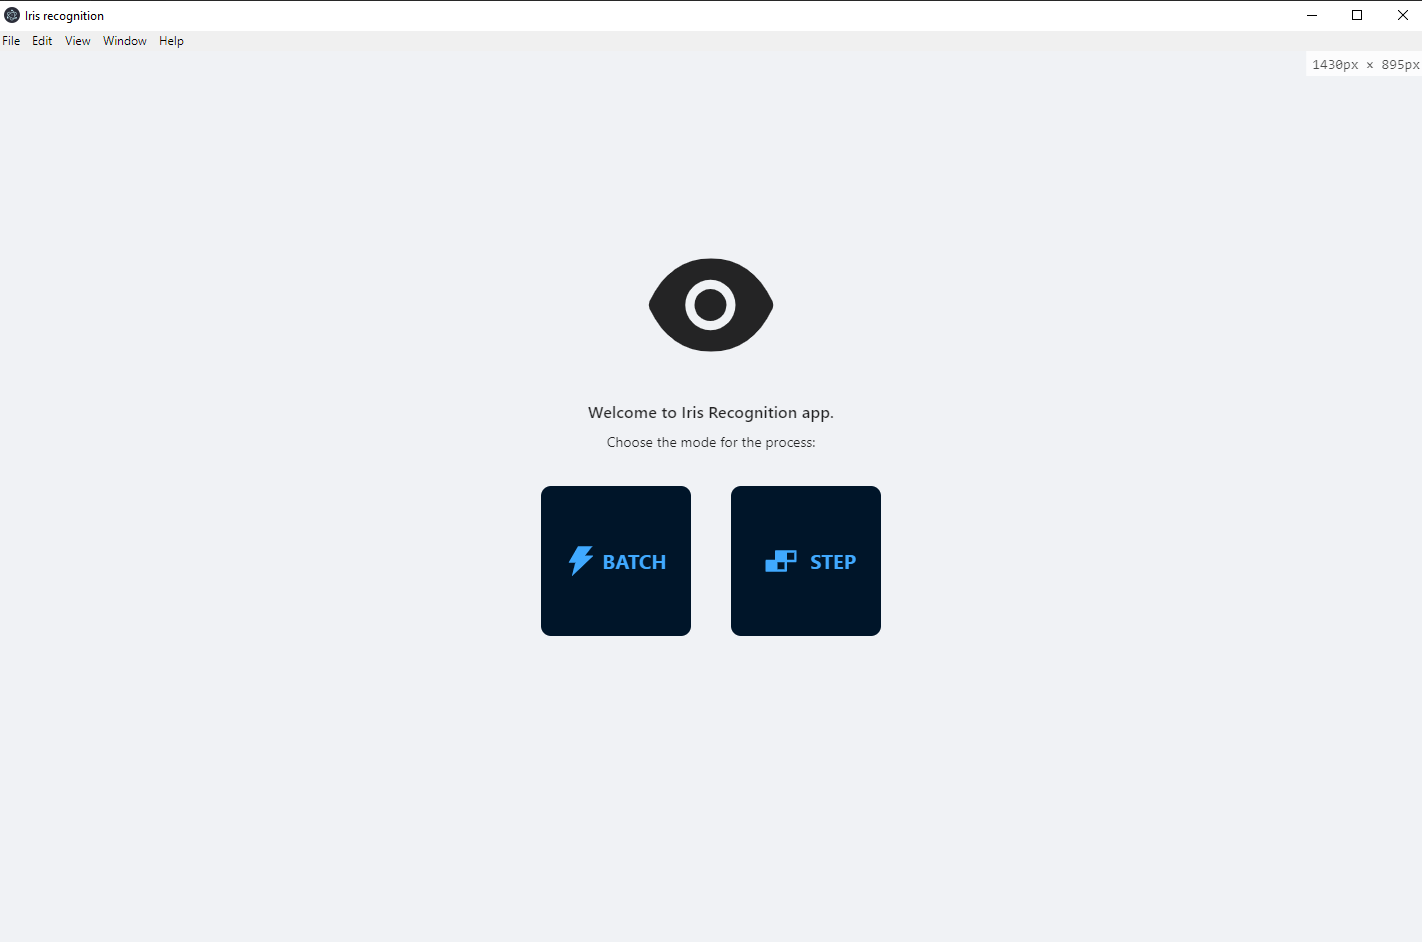
\includegraphics[width=0.8\textwidth]{images/app/home.png}
  \caption{Zrzut ekranu widoku startowego.}
  \label{fig:homeScreen}
\end{figure}

\begin{figure}[ht]
  \centering
  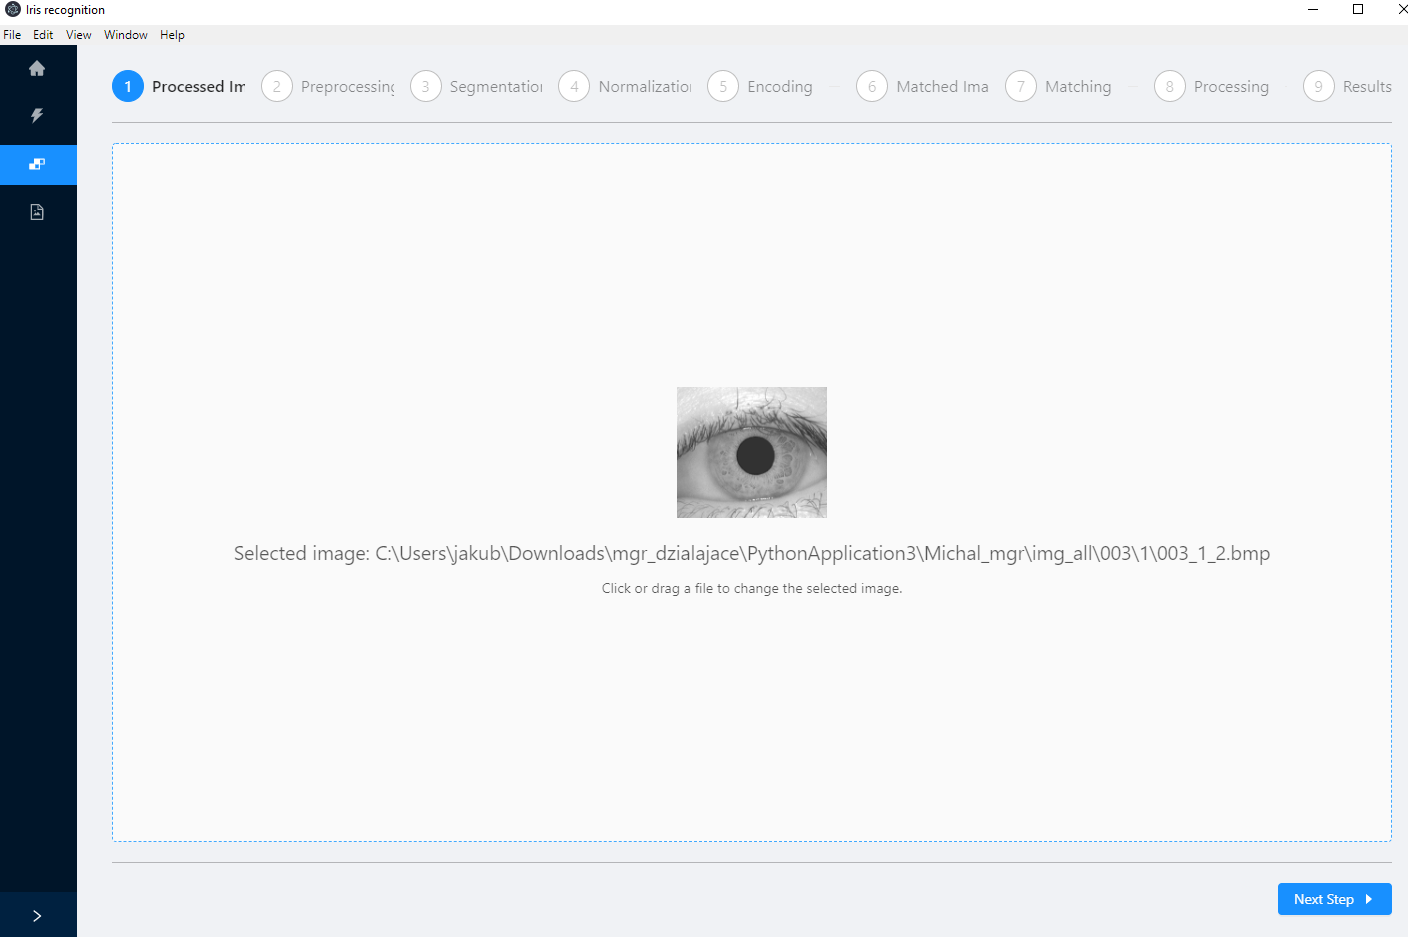
\includegraphics[width=0.8\textwidth]{images/app/step1.png}
  \caption{Widok wyboru obrazu poddawanego procesowi.}
  \label{fig:processingImageSelectionScreen}
\end{figure}

\begin{figure}[ht]
  \centering
  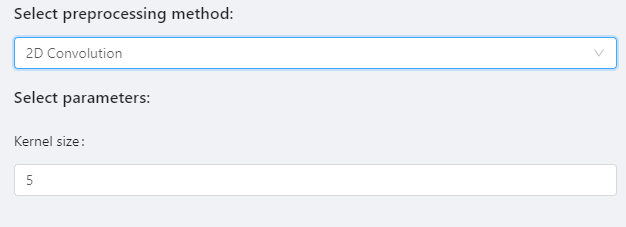
\includegraphics[width=0.7\textwidth]{images/app/preprocessingOtherMethod.png}
  \caption{Zmiana dostępnych paramterów po zmianie wybranej metody.}
  \label{fig:preprocessingOtherMethod}
\end{figure}

\begin{figure}[ht]
  \centering
  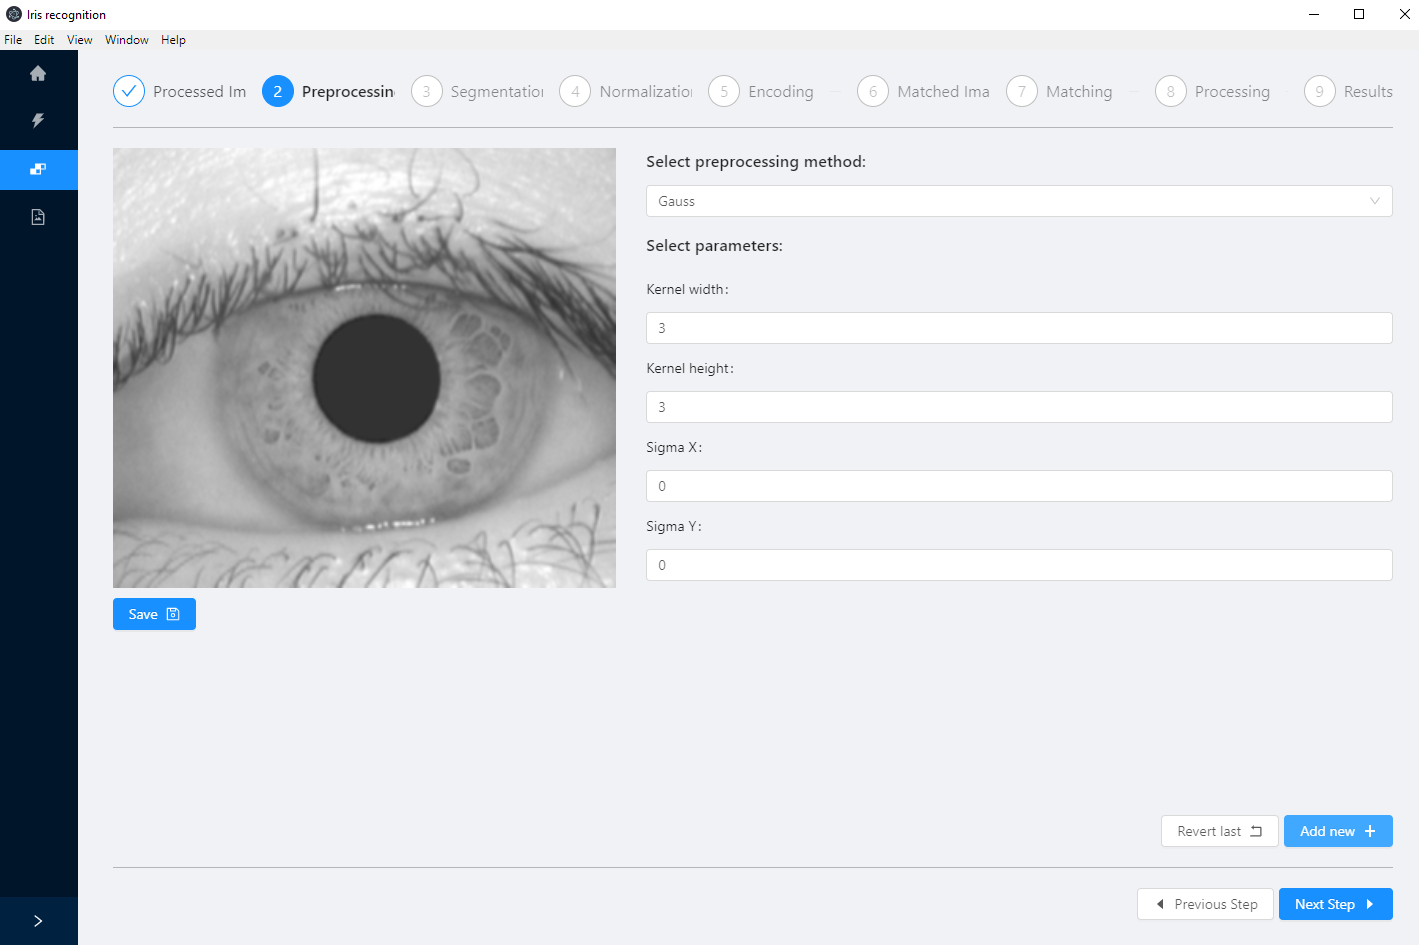
\includegraphics[width=0.8\textwidth]{images/app/preprocessing.png}
  \caption{Widok kroku przetwarzania wstępnego.}
  \label{fig:preprocessingScreen}
\end{figure}

\begin{figure}[ht]
  \centering
  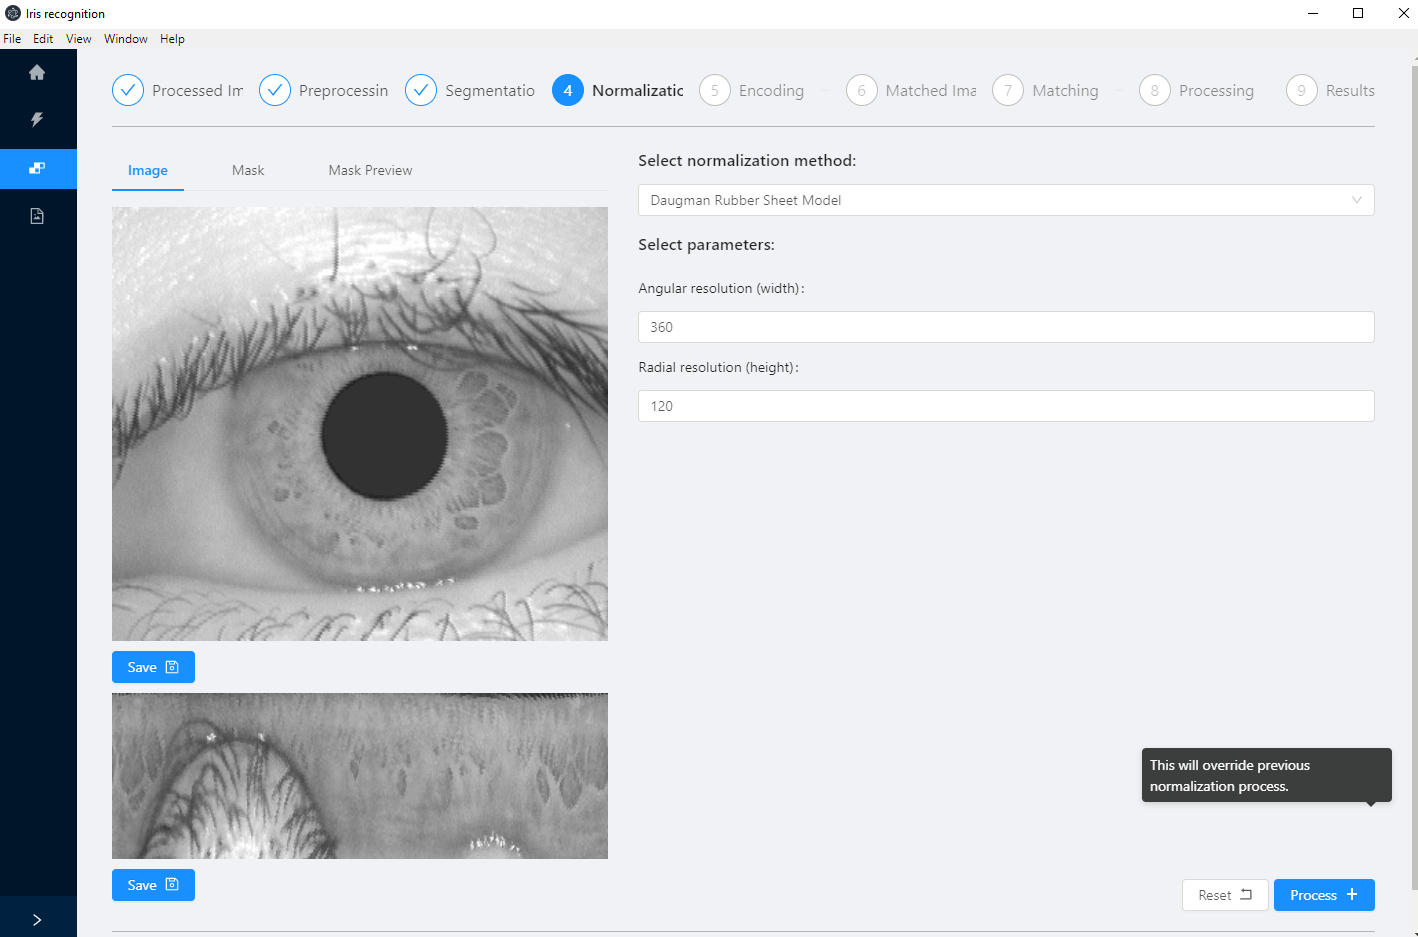
\includegraphics[width=0.8\textwidth]{images/app/normalization.png}
  \caption{Zrzut ekranu widoku procesu normalizacji.}
  \label{fig:normScreen}
\end{figure}

\begin{figure}[ht]
  \centering
  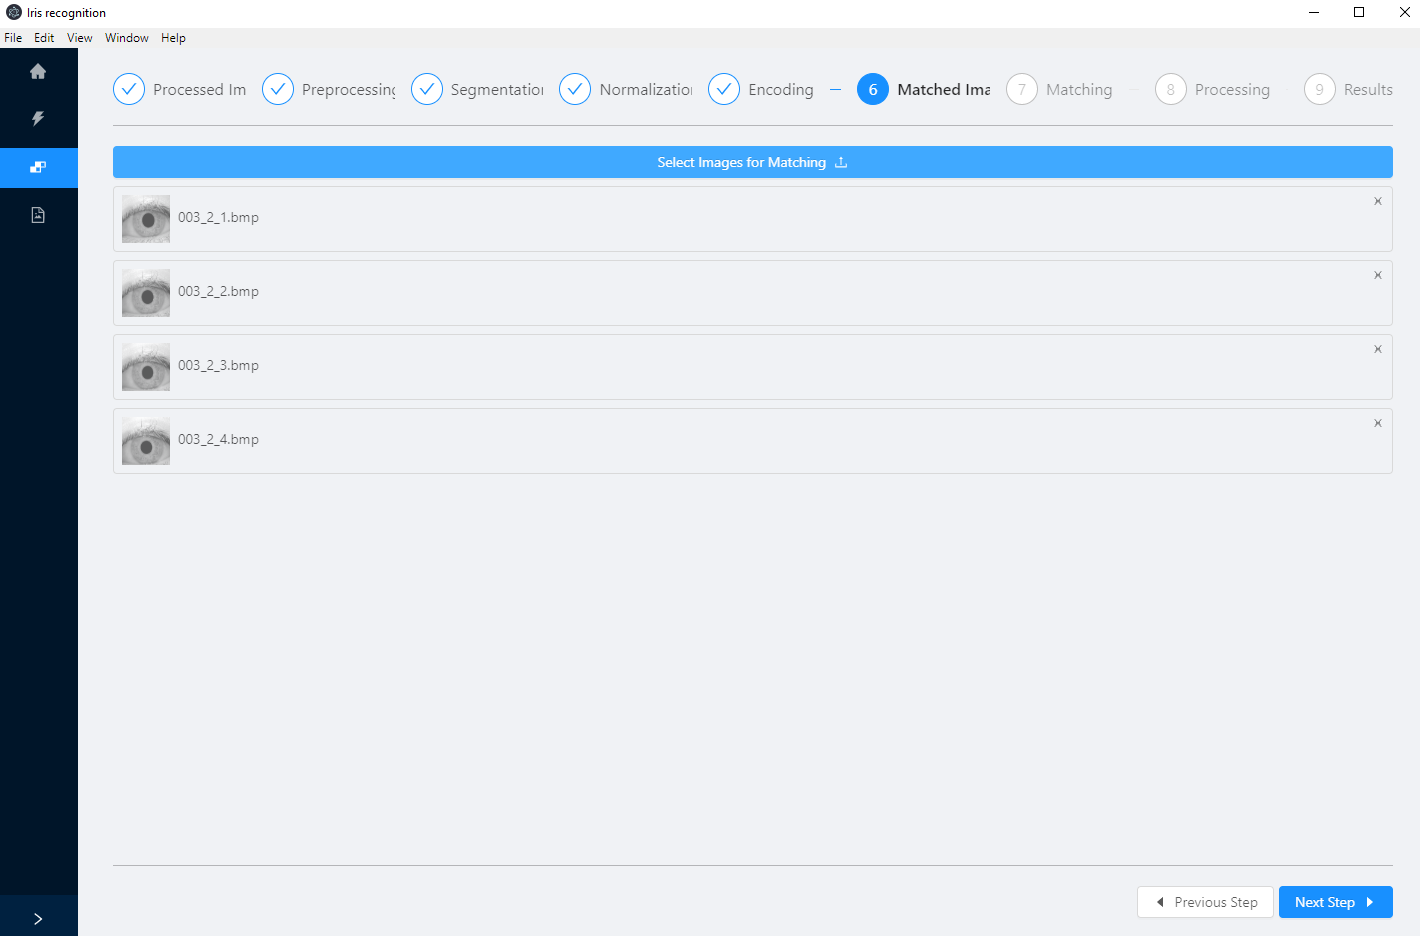
\includegraphics[width=0.8\textwidth]{images/app/matchingImages.png}
  \caption{Wybór obrazów do których chcemy dopasowa\'c przetwarzany obraz.}
  \label{fig:matchingImagesScreen}
\end{figure}

\begin{figure}[ht]
  \centering
  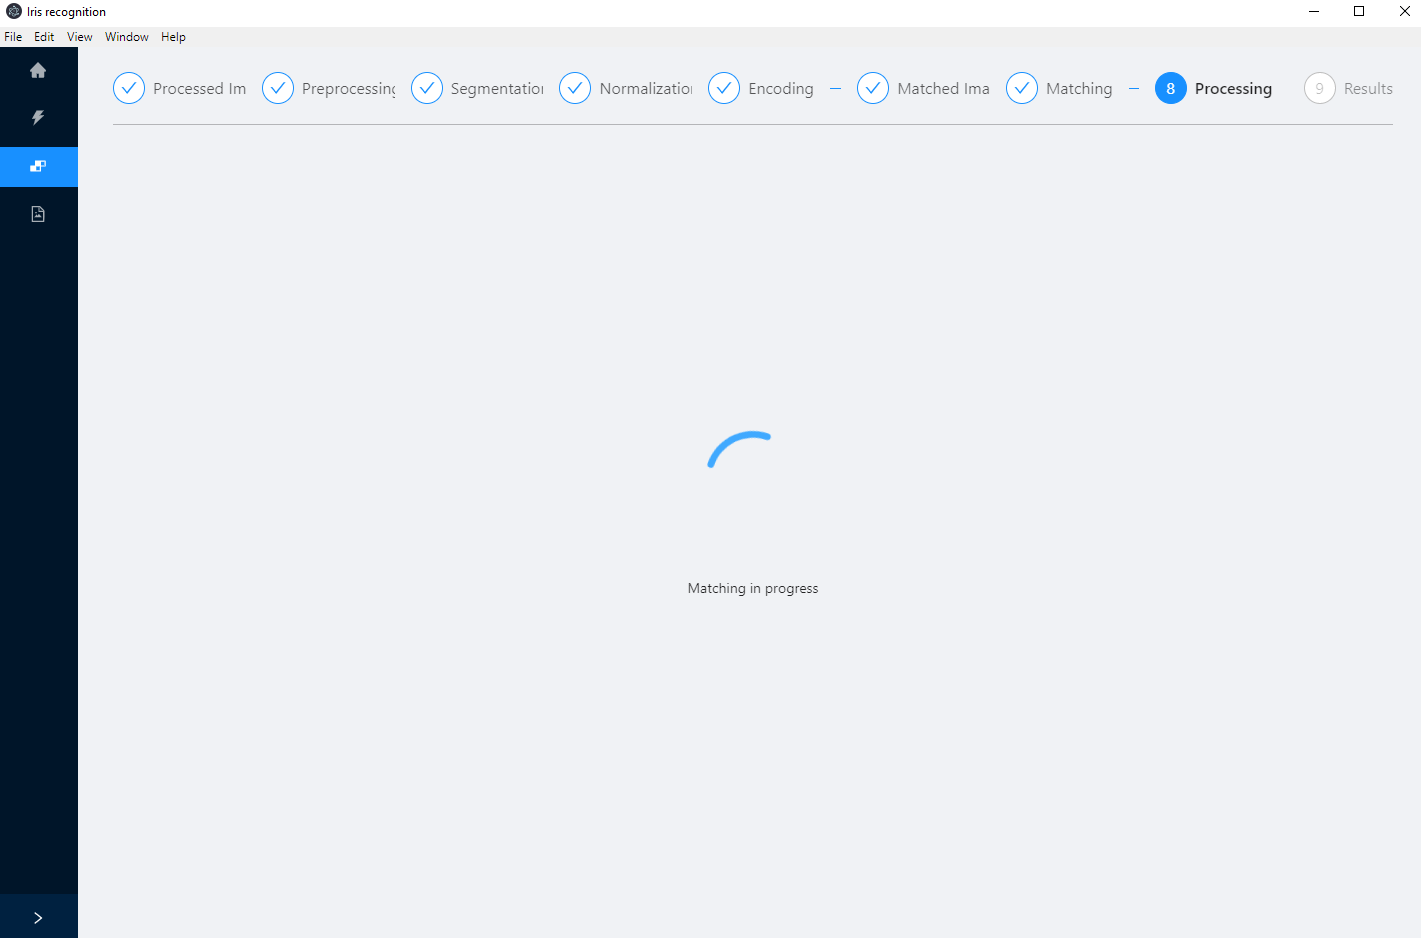
\includegraphics[width=0.8\textwidth]{images/app/matchingProgress.png}
  \caption{Widok podczas przetwarzania obrazów oraz dopasowania.}
  \label{fig:matchingProcessing}
\end{figure}

